\documentclass[UTF8]{ctexart}
\usepackage[a4paper,left=3cm,right=3cm,top=1.2cm]{geometry}
\usepackage{amsmath}
\usepackage{enumitem}
\usepackage{float}
\usepackage{threeparttable}
\usepackage{caption}
\usepackage{multirow}
\usepackage{graphicx}
\usepackage{listings}
\usepackage{color}
\usepackage{amssymb}
\usepackage{algorithm}
\usepackage{algorithmicx}
\usepackage{algpseudocode}  
\usepackage{amsmath}  
\renewcommand{\algorithmicrequire}{\textbf{Input:}}  % Use Input in the format of Algorithm  
\renewcommand{\algorithmicensure}{\textbf{Output:}} % Use Output in the format of Algorithm  
\definecolor{dkgreen}{rgb}{0,0.6,0}
\definecolor{gray}{rgb}{0.5,0.5,0.5}
\definecolor{mauve}{rgb}{0.58,0,0.82}
\lstset{frame=tb,
  language=Python,
  aboveskip=3mm,
  belowskip=3mm,
  showstringspaces=false,
  columns=flexible,
  basicstyle={\small\ttfamily},
  numbers=left,%设置行号位置none不显示行号
  %numberstyle=\tiny\courier, %设置行号大小
  numberstyle=\tiny\color{gray},
  keywordstyle=\color{blue},
  commentstyle=\color{dkgreen},
  stringstyle=\color{mauve},
  breaklines=true,
  breakatwhitespace=true,
  escapeinside=`,%逃逸字符(1左面的键),用于显示中文例如在代码中`中文...`
  tabsize=4,
  extendedchars=false %解决代码跨页时,章节标题,页眉等汉字不显示的问题
}

\setlength\lineskiplimit{5.25bp}
\setlength\lineskip{5.25bp}

\title{编程作业一实验报告}
\author{崔士强 PB22151743}
\date{\today}

\bibliographystyle{plain}

\begin{document}

\maketitle
\section{算法}

\begin{figure}[h]
  \centering
  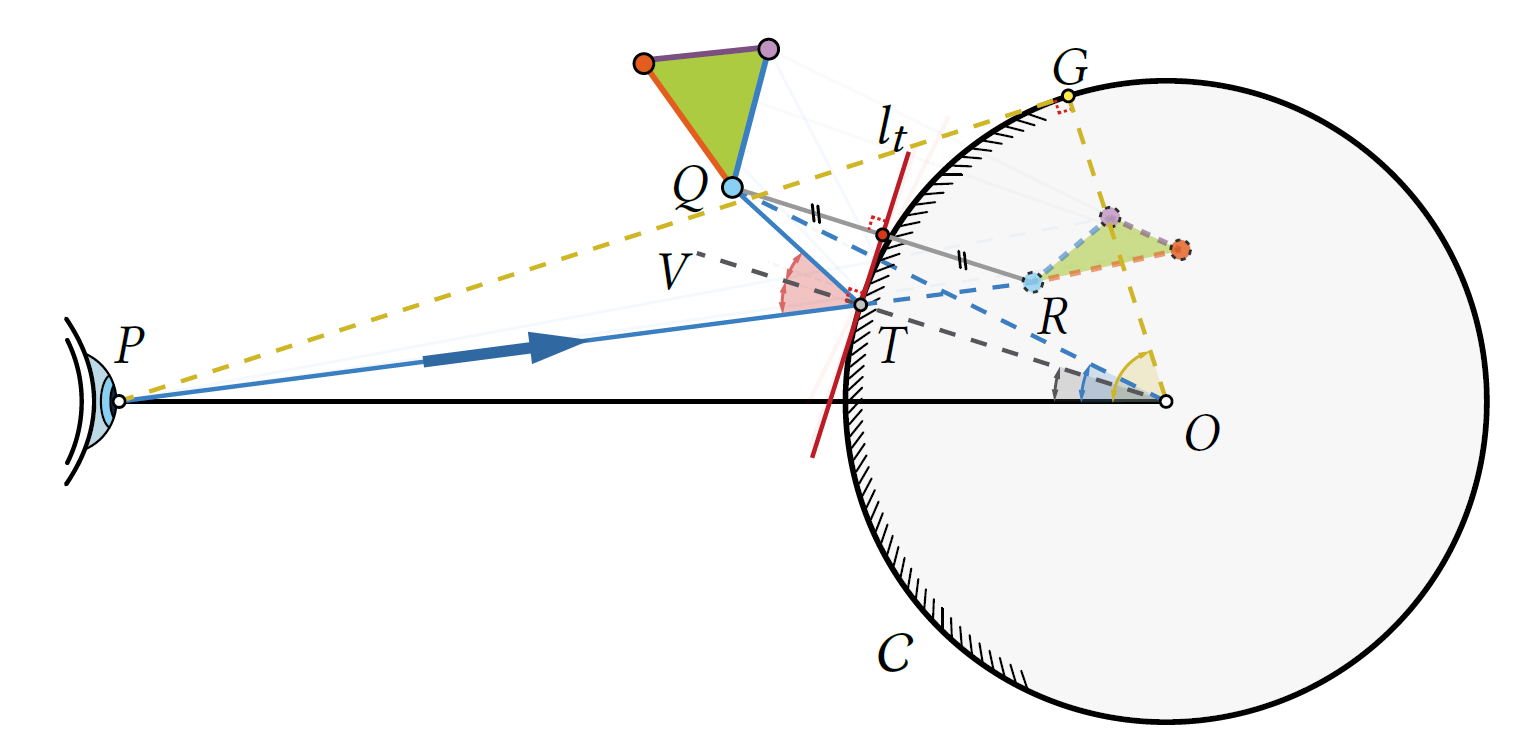
\includegraphics[scale=0.15]{pic.png}
  \caption{示意图}
\end{figure}

在Computational Mirror Cup and Saucer Art中有以下结论:

当$\angle POT$从$0$增加到$\min{\angle POQ, \angle POG}$时,
其中$G \in \mathbb{C}$且满足$PG \perp OG$,$\angle PTV$严格增加
而$\angle QTV$严格减小,并且$\angle PTV - \angle QTV$从负值严格增加到正值.

因此,我们可以采用二分法找到点$T$, 使得$\angle PTV - \angle QTV = 0$. 以$\angle POQ$为上界,$0$为下界,取
角平分线,若$\angle PTV - \angle QTV > 0$,则取左半边,否则取右半边,直到$\angle PTV - \angle QTV$足够小.

\begin{algorithm}[H]
  \caption{Binary search for $T$}
  \begin{algorithmic}[1]
    \Require
      $x_P, x_Q, y_Q$
    \Ensure
      $T \in \mathbb{C}$, $\angle PTV - \angle QTV = 0$
    \State $l \gets 0$
    \State $r \gets \angle POQ$
    \While {$\angle PTV - \angle QTV > \varepsilon$}
      \State $m \gets (l + r) / 2$
      \If {$\angle PTV - \angle QTV > 0$}
        \State $l \gets m$
      \Else
        \State $r \gets m$
      \EndIf
    \EndWhile
    \State \Return $T$
  \end{algorithmic}
\end{algorithm}

找到$T$后,通过延长$PT$可以找到$R$,延长的长度为$QT$

\section{实验结果}
实验中对8个测试样例进行计算,
通过\lstinline{np.set_printoptions(precision=20, suppress=True)}设置输出精度以及格式. 
上述算法中$\varepsilon = 10^{-8}$. 程序实现中使用递归实现二分法查找,输出结果包括递归深度,$T, R$的坐标以及
每个样例的计算时间. 结果如下图所示:
\begin{figure}[H]
  \centering
  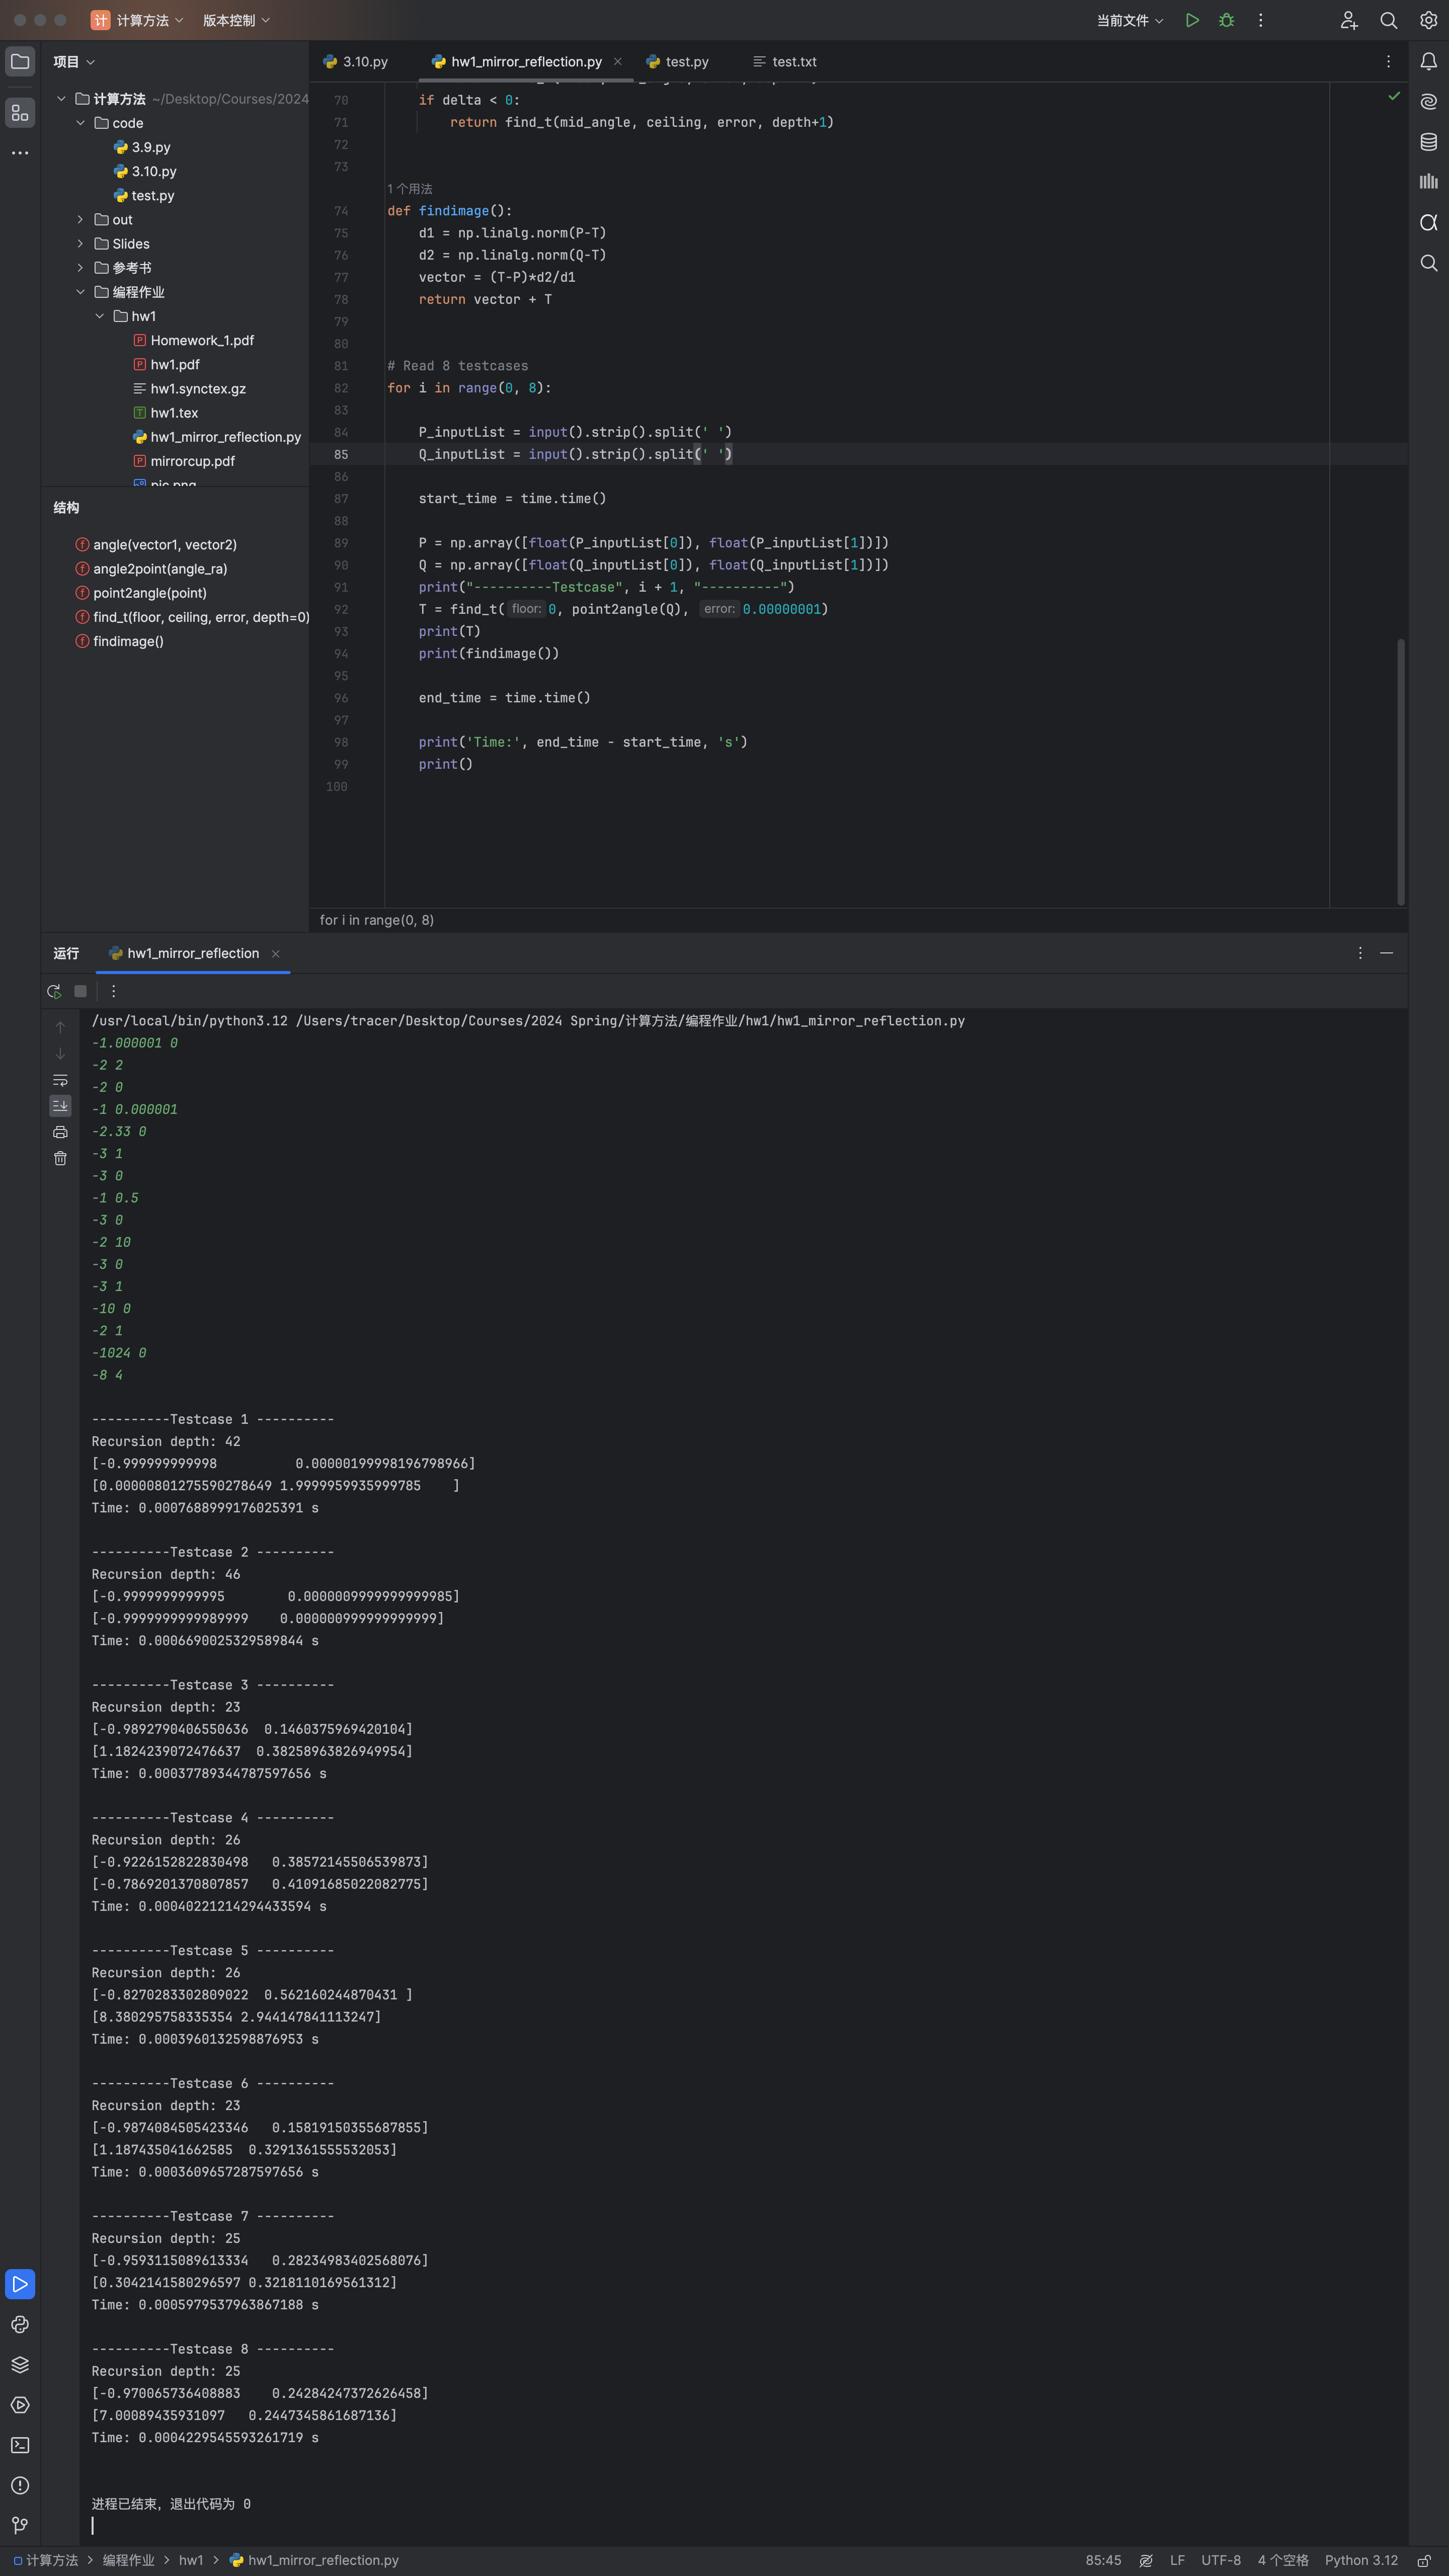
\includegraphics[scale=0.23]{test.png}
  \caption{计算结果}
\end{figure}

\section{实验分析}
\subsection{精确度}
本算法的精度问题主要来自于二分法中设置的判定阈值$\varepsilon$以及\lstinline{int}类型
的精确度. 
\subsection{稳健性分析}
\begin{enumerate}
  \item 此程序并未对不合法输入进行处理,默认输入的两个点符合规则
  \item 对于边缘情况,程序中通过提高输出精度的方法保证结果准确度. 可以看到对于边缘情况的处理需要更多层的递归.
\end{enumerate}

\bibliography{math}

\end{document}
\iffalse
\begin{figure}[h]
    \centering
    \includegraphics[scale=0.5]{name.png}
    \caption{name}
\end{figure}
\fi
